% Chapter 5

\chapter{Case Study: An R Inliner} % Main chapter title

\label{Chapter5} % For referencing the chapter elsewhere, use \ref{Chapter2} 

%----------------------------------------------------------------------------------------

% Define some commands to keep the formatting separated from the content 
\newcommand{\keyword}[1]{\textbf{#1}}
\newcommand{\tabhead}[1]{\textbf{#1}}
\newcommand{\code}[1]{\texttt{#1}}
\newcommand{\file}[1]{\texttt{\bfseries#1}}
\newcommand{\option}[1]{\texttt{\itshape#1}}

%----------------------------------------------------------------------------------------
This Chapter presents experimental results obtained for the RJIT OSR.
The first section describes an implementation of a speculative inliner tool, implemented inside the RJIT compiler, that relies on OSR exits to preserve the program's correctness.
The second section presents benchmarking results obtained while evaluating the OSR Inliner, and RJIT OSR main features, i.e., the compensation code to replace invalidated functions, and the \textit{getFreshIR} function.\\

\section{A speculative inliner for RJIT}
\subsection{Justification}
%Dynamic language R 
%function's can be redefined in R, need the OSR typical static opt that is not possible in R
%Used in other papers.
%interesting because implies that we need to clone IR -> put some pressure on our additions.
R is a dynamic language. 
Dynamic programming languages have the particularity to perform, at runtime, common programming behaviors executed during the compilation in static programming languages.
Extending the program, adding code, extending objects and definitions, type setting or modifying the type system are such behaviors that, in dynamic programming languages, can take place at runtime.
These particularities make certain common static compilation optimizations hard to implement in a dynamic language.
One example of such optimization is inlining (i.e., inline expansion), that replaces a function call site with the callee's body.\\

Chapter \ref{Chapter2} presents the on-stack replacement(OSR) mechanism.
OSR techniques enable to implement \textit{speculative} optimizations, i.e., to transform a function based on the assumption that the result of the transformation will be correct and improve the program's performance at runtime.
If the assumption fails, the OSR mechanisms preserve correctness in the program.
Thanks to this versatile tool, static programming languages optimizations can be performed speculatively in a compiler for a dynamic programming language.\\

In R, and more specifically in RJIT, inlining functions is hard. 
An R function is wrapped in a closure, and might be redefined at any time during the program's execution.
As a result, the only viable way of allowing function inlining in RJIT is to rely on OSR mechanisms.\\

Inlining is an interesting optimization, and its impact on the code performance is hard to predict. 
It holds an important trade-off between time and space, i.e., how much improvement in terms of speed can be obtained, at the cost of some extra space.
Furthermore, excessive inlining might increase register pressure and deplete the instruction cache, therefore decreasing the speed of the program's execution.
Finally, inlining can be viewed as a first step toward other optimizations.
Copying a function's body at its call site enables to enlarge the scope considered by the compiler, and might therefore uncover new optimization opportunities.\\

Apart from being a viable OSR-based speculative optimization in RJIT, inlining allows to put some pressure on the OSR Handler's mechanisms.
First, as explained in Chapter \ref{Chapter4New}, the OSR mechanism requires to obtain fresh clones of functions bodies via the OSR Handler's functions.
Second, in order to inline a function call, a copy of the callee's body needs to be obtained.
This body, in RJIT OSR, can be obtained through the OSR Handler API.
Function inlining might further force AOT compilation of the inlined functions, hence enabling us to test every aspect of the functionalities provided by the OSR Handler.\\

RJIT does not gather profiling information that enable to identify good candidates for inlining.
This is, however, far from being a limitation.
On the contrary, it is a perfect case study for OSR mechanisms in R.
Although inlining function calls in R produces unsound compiled code, the OSR mechanism enables to ensure that the program is correct.
As explained in Section \ref{justificationgoals}, R performance bottlenecks are consequences of the language semantics.
In the future, on-stack replacement is destined to enable to break R semantics, and to produce unsound, highly optimized code.
Profiling will give insights on whether or not the program might benefit from such optimizations, but is not expected to be able to ensure that any of these transformations is sound.
Not relying on a profiler and blindly inlining function calls, whenever it is possible, shows how much flexibility this OSR implementation truly brings to RJIT.\\ 

\subsection{Challenges}
%Function Calls -> how to identify them
%Resolving the function
%Continuation function problem
%IR fresh + AOT behavior
%TODO ENVIRONMENT !!!!!!!!
An OSR-based speculative inliner for RJIT needs to be implemented at the LLVM IR level.
This requires to identify function calls inside the LLVM IR, extract the callee's SEXP from the environment, and perform the appropriate transformations on the IR.
While relatively simple conceptually, implementing such a mechanism presents several challenges in RJIT.\\

An R function call corresponds to several instructions in the RJIT LLVM IR.
First, a call to the \textit{getFunction} intrinsic is inserted.
The call takes as parameter the AST of the call, stored in the constant pool associated to the function SEXP.
This intrinsic enables to resolve, at runtime, the callee. 
To do so it explores the current environment.
If no match is found, it accesses the enclosing environments until either reaching a definition or triggering an error letting the user know that the callee could not be found.
The compiler then emits instructions to load arguments to the function call.
Finally, an ic stub is generated. 
The ic stub takes as arguments the result of the call to the \textit{getFunction} intrinsic, the arguments provided to the call, a pointer to the caller, the current constant pool, and the environment.
When executed once, the ic stub replaces itself with a call to an inlined cached wrapper function dedicated to the callee.
Figure \ref{fig:functioncall} provides a simple R function that performs a function call, and the equivalent LLVM IR generated by RJIT.
Line 5 resolves the callee closure from the environment, line 6 loads the argument to the call, and line 8 performs the call to the ic stub.\\

In the OSR inliner, function calls can be identified by looking for ic stubs.
The OSR inliner has to run on non-instrumented LLVM IR. 
The ic stubs have not yet been replaced by inlined cached wrappers.
Therefore, even though a function call is compiled into several instructions, ic stubs and their arguments are enough to obtain all the information corresponding to a function call.\\

\begin{figure}[h]
\includecode{Code/functionCall.c}
\caption{Example of RJIT LLVM IR for a function call.}
\label{fig:functioncall}
\end{figure}


The OSR inliner needs to obtain a clone of the callee's LLVM IR, in order to inline a function call.
If the callee was never compiled before, the \textit{getFreshIR} function will trigger an AOT compilation of the function.
Since the OSR inliner heavily relies on fresh IR, one challenge is to try to minimize the amount of cloning required in order to perform the transformations.\\

Inlining in R requires to create a dedicated environment for the inlined function.
Implementing a sound name mangler in R is hard. 
It requires to check that fresh names do not collide with parent or child environments.
Furthermore, replacing arguments with their actual values is not semantically correct, due to the way promises are evaluated.
For these reasons, creating a dedicated environment appears to be the only sound solution.\\

The OSR Kit mechanism requires to associate a \textit{toInstrument} clone to every function transformed.
The continuation function has to be a clone of the base function used to generate the optimized one.
One challenge is to carefully implement the inlining in order to limit the number of \textit{toInstrument} functions generated.\\

Finally, all the challenges related to the cloned and continuation functions mentioned in Section \ref{additionalchallenges} need to be considered.
Fixing the LLVM IR requires to go through every instruction in the cloned functions.
As a result, in order to save compilation time, it is important to perform such operations only when they are truly needed.\\

\subsection{Implementation}
%FunctionCall to abstract away the call
%The different mods for inlining.
%The algorithm to inline.
MORE MODES OF EXECUTION !!!!!\\

This section describes the implementation of the OSR inliner.
The OSR inliner relies on a special C++ class, called \textit{FunctionCall}, to extract function calls in the LLVM IR and easily access its elements. 
The OSR inliner also provides different modes of execution, that enable more or less aggressive speculative inlining.\\

The FunctionCall class provides a static function, called \textit{getFunctionCalls}, that takes an LLVM IR as input, and extracts the function calls it contains.
For each ic stub call, the function creates an instance of the FunctionCall class. 
A FunctionCall object gives quick access to each element of the function call, i.e., the \textit{getFunction} call instruction, the arguments to the call, and the additional elements of the ic stub call.
The \textit{getFunctionCalls} returns a list of FunctionCall instances.
It is important to note that, for efficiency and better integration, the \textit{getFunctionCalls}, or any similar function that needs to go through the LLVM IR instructions and match a specific pattern, will be able to rely on the pass \& match mechanism being developed in RJIT.
RJIT provides a special matcher mechanism, combined to the LLVM passes implementation, that enables to extract special patterns from the LLVM IR.
One of its main goals is to reduce the number of iterations on the entire LLVM IR, by merging different passes.
Unfortunately, this feature was not yet ready at the time at which the RJIT OSR project was implemented.\\

The OSR inliner implements is a very basic, aggressive, speculative inlining algorithm. 
RJIT does not have a profiler or a static analyzer yet.
As a result, the OSR inliner cannot rely on any extra information to decide if a call should be inlined or not.
The OSR inliner proposes different modes of execution, that enable more or less aggressive inlining techniques.
The default mode of execution inlines all the calls inside the current function, as long as a body can be obtained for the callee.
The OSR inliner does not inline recursive calls.
A more agressive mode, called \textit{all inline}, enables to recursively apply the OSR inliner on the body of the functions being inlined.
Function calls that contain ellipsis or missing arguments are not inlined by the OSR Inliner.
\\


The OSR inliner implements a very naive inlining algorithm.
All functions calls are extracted from the outer function using the \textit{getFunctionCalls} function.
The OSR Inliner then traverses the list of function calls, and groups them by call targets.
The callee's closure can be obtained by looking up the symbol of the function call in the outer function's environment.
In the \textit{all inline} mode, the OSR inliner generates a fully inlined LLVM IR for each different callee, i.e., it inlines all the calls inside each compiled callee. 
In the default mode, the OSR inliner simply calls the getFreshIR method to obtain the callee's LLVM IR.
The OSR inliner creates the toInstrument clone of the outer function.
The toInstrument is used to create the continuation function for each OSR exit inserted in the outer function.
It is wrapped in a valid function SEXP, added to the module, and has a valid IR.
Then, for each different callee, the OSR inliner proceeds as follows: 
\begin{enumerate}
    \item In the body of the callee, update accesses to the constant pool by changing the index to $\text{LENGTH}(\text{CP}_{\text{outer}} + \text{index})$.
    \item Append the callee's constant pool to the outer function's one.
    \item For each function call to the callee:
        \begin{enumerate}
            \item Obtain an unused clone of the callee.
            \item Insert instructions to create a new environment that contains the correct arguments to values mappings, before the ic stub.\label{step:newrho}
            \item Replace all accesses to the environment, i.e., rho argument, in the callee's body by the newly created environment.
            \item Move the callee's body inside the outer function, after the instruction of step \ref{step:newrho}.
            \item Replace all the callee's return instructions by forwarding the return value to a $\phi$-node inserted after the callee's body.\label{step:phinode}
            \item Remove the ic stub.
            \item Replace the ic stub in the transitive mapping between the toInstrument and the outer function by a mapping between the toInstrument corresponding ic stub and the $\phi$-node created in step \ref{step:phinode}.\label{step:updatemap}
            \item Call the insertOSRExit with the outer function as the from function, the toInstrument as the continuation function, instructions that compare the result of the \textit{getFunction} call with the hard coded address of the callee's closure as the OSR condition, and the \textit{constant} call as the transition point, i.e., the instruction that was directly above the ic stub in the original outer function.
        \end{enumerate}
    \item Call the \textit{resetSafePoints} function to correct the optimized function's IR.
    \item Set the optimized function SEXP inside the closure.
    \item Add the optimized function SEXP to the relocations.
    \item Return the closure.
\end{enumerate}

It is important to note that the OSR inliner forces the compilation of every callee. 
As a result, any function contained in the outer function, and inlined, will also be compiled. 
When in the \textit{all inline} mode, they are also fully inlined.
Any subsequent call to a callee will therefore benefit from either a fully compiled, or a fully inlined and compiled version of the function.\\

The continuation function for an OSR exit corresponds to the fully unoptimized base function. 
The toInstrument function is used to generate the continuation function and does not contain any inlined call.
This enables to limit the number of toInstrument functions generated during the transformation of the outer function and avoid triggering OSR exits in cascade.
This also illustrates that, even though it does not correspond to the behavior encouraged by the OSR Kit library, a few careful updates (step \ref{step:updatemap}) to the transitive map enable to preserve a mapping between a base function, and a working copy being modified.
On the other hand, ideally, the continuation function should inline all calls that did not fail.
This solution can be implemented with on-the-fly compilation of the continuation function, but is not provided in this prototype.\\

The OSR Inliner provides a compensation code generator mechanism. 
The compensation code is a simple call to a C++ function, that takes as argument an integer identifier.
The identifier corresponds to a function SEXP containing the toInstrument version.
The C++ function uses the identifier to retrieve the toInstrument function SEXP, and replaces the invalidated function in the closure with this SEXP.\\

CODE EXAMPLE OF INLINING, TOINSTRUMENT AND CONT.\\

\section{Tests}
\subsection{GNUR RJIT vs. Inlining on Shootout benchmarks}

\subsection{OSR Exit vs. Replacing the closure}
%OSR Handler enables to replace the continuation
%Avoids triggering the exit all of the time. 
%Need to see if this really improves performances. 
%Should be ...
The OSR Handler enables to add compensation code at the beginning of continuation functions, and replace the invalidated version with a correct one.
This mechanism allows to avoid triggering the OSR exit every time the function is executed.
The cost of an OSR exit corresponds to the cost of the OSR condition, and the function call to the continuation function.\\

In simple examples, this cost can be neglected.\\ 

\subsection{OSR Handler getFreshIR vs. Parsing the AST}
%Role of the OSR Handler getFreshIR 
    %Avoid translation step from AST to LLVM IR every time a fresh IR needs to be otbained 
    %Supposed to be faster than walking the AST and generating the llvm ir instructions.
    %Still has some expensive cost, i.e., registering a copy during first compilation, cloning to get a working copy, fixing the IR.
    %Hence need to evaluate its performances.
    %Rely on shootout benchmarks, instrumented such that each function (i.e., 172 functions) is used.

%Overall execution
    %Cost of the registering the working copy 
        %Less than half of the cost of generating  the IR. 
        %Not significant compared to the jitAll cost, i.e., final step to generate the native code.

%Case when the OSR Handler contains a clone for each function.
    %That is the true use case, i.e., functions are jitted, executed. Hot functions are then promoted for optimizations. 
    %Compare time required to parse AST and generate the LLVM IR, and the the time required to get a Fresh and correct IR via the OSR Handler. 
    %Benchmarks are instrumented to have all possible instructions invalidated in the clone, i.e., worst case. 
%Results show that the ratio between getting the working copy and the "translation" is constant, does not vary with the number of instructions in the IR, and is arround 0.33, i.e., it is 3 times faster to get the IR via the OSR Handler than to generate it by reparsing the AST.
%Provide an histogram that represents the frequency of the observed costs for obtaining the IR using both techniques.
%See that with the OSR handler, the costs are concentrated between lalalala. 

The OSR Handler, via the \textit{getFreshIR} and its utilities functions, enables to obtain a fresh, non-instrumented, and correct LLVM IR for a function.
This is meant to avoid the translation step from ASTs to LLVM IR every time a fresh non-instrumented IR is needed, e.g., for optimizations.
Obtaining a fresh IR via the OSR Handler, for an already compiled function, is supposed to be faster than walking the entire function's AST and re-generating the corresponding LLVM IR instructions.
The OSR Handler, however, performs some expensive operations, with non-negligible costs, such as registering a copy of the function in the base version map during the function's first compilation, cloning the base version entry to obtain a fresh working copy, and fixing the LLVM IR of clones.
As a result, we evaluate the OSR Handler's mechanisms performance, compared to a regular translation from ASTs to LLVM IR.
To do so, we rely on the Shootout benchmarks\cite{Shootout}, instrumented such that each function in the benchmarks is used.\\

Registering an entry in the base version map increases the cost of a function's first compilation.
A first experiment therefore consists in comparing the cost of this first compilation via the OSR Handler, and via the regular RJIT mechanism. 
Unsurprisingly, the OSR Handler exhibits poorer performances. 
The reason is that it has to generate the LLVM IR corresponding to the function's AST, as well as cloning the obtained IR and registering the clone in the base version map, hence introducing an overhead of VALUE compared to the RJIT compilation.
CONTINUE\\


The OSR Handler is supposed to improve the RJIT's performances in the presence of optimizations re-compilations.
The expected execution flow is that functions a jitted, and executed. 
When a function becomes hot, i.e., when it has been executed several times, it becomes a candidate for re-compilation and optimizations.
This corresponds to the real use case of the OSR Handler's mechanisms.
As a result, we need to evaluate the cost of obtaining a fresh and correct IR from the OSR Handler, when the base version map already contains an entry for the function, and compare it to the cost of generating the IR from the AST.
We therefore perform a second experiment, where the OSR Handler has a fully generated base version map.
In this experiment, we further ensure that every call instruction inside the clones obtained via the \textit{getFreshIR} function need to be fixed.
This corresponds to the worst case scenario for the execution of the \textit{resetSafepoints} function, and thus provides an upper bound on the performance evaluation.\\

Our second experiment yields encouraging results.
A first observation is that the time ratio between obtaining the IR via the OSR Handler and via RJIT translation is constant, regardless of the number of LLVM IR instructions generated, with a median value at \textbf{0.33}. 
In other words, it seems that obtaining a fresh and correct IR, for an arbitrarily sized function, via the OSR Handler, is in average at least \textbf{three} times faster than generating it from the AST.
These results can further be improved if less instructions need to be fixed.
As explained in Section \ref{section:cleanerIR}, a future solution would be to save an entire module per function in order to avoid having to fix LLVM IR instructions.
With this solution, the cost of obtaining a fresh non instrumented IR would include the cost of loading an LLVM module into the current compilation module. 
Since it is not part of our implementation, we do not provide any estimation for this cost.\\

\begin{figure}[h]
    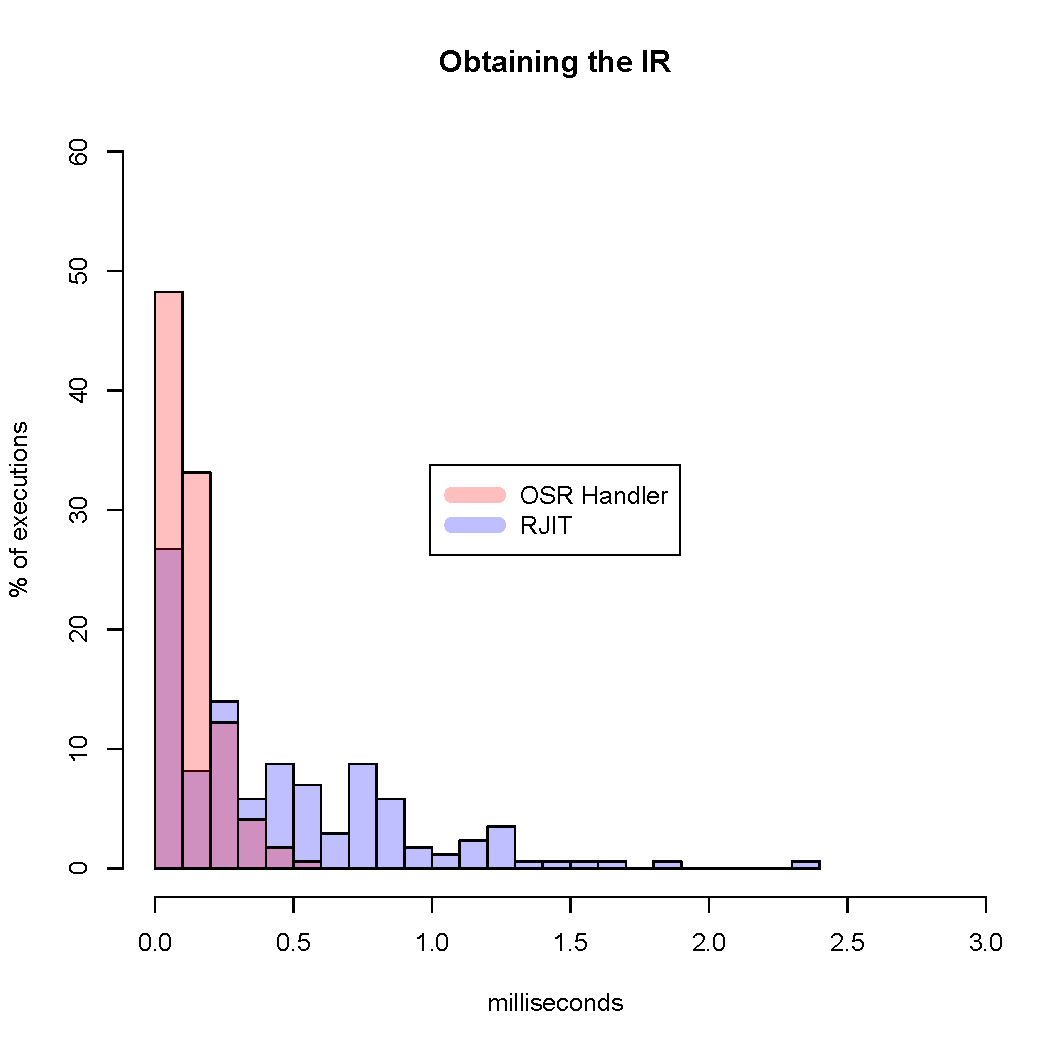
\includegraphics[scale=1]{Figures/withoutJitAll}
    \caption{OSR Handler vs. RJIT: histogram of the time required to obtain a fresh and correct IR for all the functions in the Shootout benchmark.}
    \label{fig:withoutJitAll}
\end{figure}

Figure \ref{fig:withoutJitAll} presents an histogram corresponding to our second experiment.
The histogram represents the distribution of times observed to obtain a fresh, non-instrumented, and correct IR, via RJIT and via the OSR Handler, on the same set of functions.
For the OSR Handler, all values are contained between X and X.
HOW TO COMMENT PROPERLY AN HISTOGRAM.\\

CONCLUDE\\
